\documentclass[journal]{IEEEtran}

\usepackage{amsmath,amssymb,amsfonts}
\usepackage{graphicx}
% Figure search path: repo layout (../results/figures) or a flat upload (figures next to the .tex).
\graphicspath{{../results/figures/}{figures/}{./}}
\usepackage{textcomp}
\usepackage{booktabs}
\usepackage{multirow}
\usepackage{cite}
\usepackage{hyperref}
\usepackage{url}
\usepackage{bm}
\usepackage{mathtools}
\usepackage{amsthm}
\newtheorem{proposition}{Proposition}

% Public code + data repository (single source of truth)
\newcommand{\repourl}{https://github.com/Praveg432/OmniST}

\begin{document}

\title{OmniST: Topology-Invariant Forecasting for Dynamic Sensor Networks With Guaranteed Coverage
at Unseen Sensors}

\author{Praveg~Vashishtha
\thanks{P. Vashishtha is with the Department of Computer Science and Engineering, Indian Institute
of Technology Patna, India, and with Sopra Banking Software India, where he is a Senior Software
Development Engineer (e-mail: praveg\_pa2503mth259@iitp.ac.in).}}

\maketitle

\begin{abstract}
Deployed sensor networks change: stations are added, fail, or go offline for maintenance. Graph
convolutional forecasters built on a fixed adjacency matrix tie their weights to the sensors seen in
training, so they cannot forecast at a new location and they fail when sensors are removed. We
present OmniST, a forecaster with no structural dependency on the number of sensors. Each sensor is
embedded from its geographic coordinates, spatial context comes from nearest-neighbor attention
recomputed at every forward pass, and each sensor's history is processed independently. Combined with
inductive split-conformal calibration, OmniST returns distribution-free prediction intervals with a
finite-sample coverage guarantee at sensor locations never seen in training. We show that a sensor's
nonconformity score is unchanged by topology changes outside its neighborhood, so in that regime the
guarantee needs no recalibration. On four real sensor datasets covering air quality, weather and
freeway traffic, coverage at unseen sensors stays at or above 90\% under 30 to 50\% sensor dropout,
while four interpolation baselines each fall short on several datasets, and it holds at 325 real
traffic sensors. At unseen air-quality stations, point error is 12\% below nearest-neighbor
interpolation and 21\% below a learned kriging network. A rolling adaptive-conformal layer restores
coverage under seasonal drift, lifting late-year coverage from 0.50 to 0.96.
\end{abstract}

\begin{IEEEkeywords}
Sensor networks, spatiotemporal forecasting, conformal prediction, uncertainty quantification,
sensor failure, inductive prediction.
\end{IEEEkeywords}

%% ====================================================================
\section{Introduction}
\label{sec:introduction}

\IEEEPARstart{A}{n} operational sensor network rarely keeps the layout it was trained on. India's
Central Pollution Control Board adds air-quality stations every year~\cite{panja2026estgcn}, traffic
detectors fail, and weather stations go offline for maintenance. A forecaster serving such a network
has to keep working when a sensor disappears, and it has to say something useful at a location where
a new sensor is planned or has just been installed.

Spatiotemporal graph convolutional networks (STGCNs)~\cite{yu2018stgcn} forecast accurately on a
fixed network, but they encode it as a pre-computed $N\times N$ adjacency matrix. A sensor added after
training has no row or column in that matrix, so the model produces no forecast there, and removing a
trained sensor breaks the matrix product. Some implementations recompute the adjacency and can adapt,
but that is an engineering choice rather than something the formulation provides.

A point forecast at a new location is also not enough for an operator. Before acting on it, they need
to know how far to trust it. This paper asks whether a forecaster can deliver both: forecasts at any
set of sensors, including unseen ones, and intervals at those sensors that carry a finite-sample
coverage guarantee which survives when the network changes.

Our answer is OmniST, a design in which no component references a global sensor count. We use
``topology invariant'' in this sense: the model produces valid outputs for any number of sensors. We
do not claim that accuracy is invariant, though it is stable in practice. The contributions are:
\begin{enumerate}
\item \textbf{Guaranteed-coverage intervals at unseen sensors.} Composing coordinate-based inductive
prediction with inductive split-conformal calibration~\cite{conformalinductivegnn2024} yields
distribution-free intervals at sensor locations with no training history. We prove a locality
property (Proposition~\ref{prop:locality}): each sensor's nonconformity score is exactly invariant to
sensors outside its neighborhood, so the guarantee needs no recalibration under far-field topology
changes.
\item \textbf{Resilience to sensor failure.} Accuracy degrades by at most 1.1\% when 40\% of
stations are removed at inference, and coverage holds under 30 to 50\% dropout, while a
fixed-topology baseline fails outright.
\item \textbf{Multi-domain validation on real sensor data.} Coverage at unseen sensors holds on four
real datasets from three physical domains (Delhi and Beijing air quality, NOAA weather, Caltrans
traffic) and at 325 real traffic sensors. Among OmniST and four model-free interpolators, only
OmniST holds the target on every dataset.
\item \textbf{Coverage over time.} A rolling-window quantile combined with Adaptive Conformal
Inference~\cite{gibbs2021aci} restores coverage under seasonal drift, where static conformal fails.
\end{enumerate}

%% ====================================================================
\section{Method}
\label{sec:architecture}

\subsection{An Architecture With No Global Sensor Count}

OmniST satisfies one invariant: for any component $f$ and any sensor $i$, $f(i)$ depends only on
sensor $i$'s own data and a fixed-size neighborhood $\mathcal{N}_k(i)$, never on the full set of
sensors present.

\textbf{Coordinate tokens.} Each observation becomes a token
\begin{equation}
\mathbf{z}_i(t) = f_{\text{MLP}}(\phi_i, \lambda_i) + f_{\text{time}}(t) + W_f \mathbf{x}_i(t),
\end{equation}
where $f_{\text{MLP}}:\mathbb{R}^2\to\mathbb{R}^d$ is a 3-layer MLP on centered latitude and longitude,
$f_{\text{time}}$ encodes calendar features with sinusoidal harmonics, and $W_f$ projects the raw
measurements. No other sensor enters $\mathbf{z}_i(t)$.

\textbf{Neighbor attention.} Spatial context comes from the $k$ geographically nearest sensors,
\begin{equation}
\mathbf{z}_i' = \text{LayerNorm}\Big(\mathbf{z}_i + \sum_{j \in \mathcal{N}_k(i)} \alpha_{ij} W_v \mathbf{z}_j\Big),
\end{equation}
where $\mathcal{N}_k(i)$ is found by Haversine distance at every forward pass and $\alpha_{ij}$ are
multi-head attention weights with a learned distance bias. When sensors are removed, the remaining
ones find their neighbors among those still reporting.

\textbf{Per-sensor temporal model and head.} A bidirectional GRU processes each sensor's sequence
independently, by reshaping the $(B,T,N,d)$ tensor to $(B{\cdot}N,T,d)$, and a 2-layer MLP maps the
final state to the forecast horizon. There is no cross-sensor operation in either. This is also why
robustness to sensor dropout is largely built in rather than learned.

The model has ${\sim}315$K parameters at $d{=}128$. Training uses AdamW with cosine annealing and
early stopping. We use the Peaks-Over-Threshold loss of~\cite{panja2026estgcn} throughout, so the
controlled comparison in Section~\ref{sec:controlled} differs only in the spatial backbone.

\subsection{Coverage-Guaranteed Intervals at Unseen Sensors}
\label{sec:conformal}

We wrap OmniST in split conformal prediction~\cite{vovk2005algorithmic,angelopoulos2023conformal}.
With absolute residuals $s_i = |\hat{x}_i - x_i|$ on a calibration set $\mathcal{C}$ of size $n$, the
half-width is
\begin{equation}
\hat{q} = \mathrm{Quantile}\!\left(\{s_i\}_{i \in \mathcal{C}},\; \tfrac{\lceil (n+1)(1-\alpha)\rceil}{n}\right),
\end{equation}
and the interval is $[\hat{x} - \hat{q},\, \hat{x} + \hat{q}]$, clipped at zero for non-negative
quantities. Under exchangeability this gives marginal coverage of at least $1-\alpha$.

In the inductive setting the calibration residuals come from training sensors while the test point
is an unseen sensor, so the calibration and test scores must remain exchangeable, the issue analyzed
for graph models in~\cite{conformalinductivegnn2024}. For message-passing GNNs this is delicate:
adding or removing any node perturbs every embedding and shifts all calibration scores. OmniST's
per-sensor construction gives an exact property instead.

\begin{proposition}[Locality implies exact score invariance]
\label{prop:locality}
Let $s_i = g\big(c_i, x_i, \{(c_j,x_j): j\in\mathcal{N}_k(i;S)\}, y_i\big)$ be the nonconformity
score of sensor $i$ given the present sensor set $S$, where $\mathcal{N}_k(i;S)$ is the set of its $k$
nearest other sensors in $S$. For any $S'$ with $\mathcal{N}_k(i;S') = \mathcal{N}_k(i;S)$, in
particular any addition or removal of sensors outside that set, $s_i(S') = s_i(S)$ exactly. Hence the
threshold $\hat q$ calibrated on training sensors remains valid without recalibration for any test
sensor whose neighbor set is unchanged.
\end{proposition}

\emph{Proof sketch.} Each component is a function of a sensor's own data and its $k$-NN receptive
field: the coordinate token depends on $(c_i,x_i)$, the attention aggregates exactly
$\mathcal{N}_k(i;S)$, and the GRU and head act per sensor. No operation uses $N$, a sensor index, or a
reduction across sensors, so $s_i$ is a fixed function of an unchanged argument. Validity of $\hat q$
then follows from standard split conformal, since neither the calibration scores nor the test score
move. $\square$

Empirically, dropping sensors outside a test sensor's neighbor set changes its prediction by less
than $10^{-7}$, while dropping a true neighbor changes it by about $7\times10^{-3}$, so the locality is
real rather than vacuous.

\subsection{Coverage Over Time}
\label{sec:online-conformal}

Split conformal is marginal under exchangeability. Over a long horizon the residual distribution
drifts with the seasons, and a quantile frozen on an early window under-covers later. We therefore
use a rolling-window quantile, which tracks the drifting residual scale, with a multiplicative
correction from Adaptive Conformal Inference (ACI)~\cite{gibbs2021aci},
\begin{equation}
\alpha_{t+1} = \alpha_t + \gamma\,(\alpha - \mathrm{err}_t),
\end{equation}
where $\mathrm{err}_t=1$ if the observation fell outside the interval at step $t$. ACI drives
long-run miscoverage to $\alpha$ for any sequence, without exchangeability. We call the combination
rolling-ACI. Its cost is wider intervals, which is unavoidable when the residuals widen.

%% ====================================================================
\section{Data and Protocol}
\label{sec:experiments}

We use four real sensor datasets from three physical domains:
\begin{itemize}
\item \textbf{Delhi air quality:} daily PM$_{2.5}$ from 37 CPCB stations (2019--2023), from the
E-STGCN public repository~\cite{panja2026estgcn}, the dataset behind its published results. This is
our primary accuracy benchmark: training on 2019--2022 (1461 days), testing on 2023 (365 days), with
60-day inputs and a 30-day horizon.
\item \textbf{Beijing air quality:} hourly PM$_{2.5}$ from the 12-station UCI Multi-Site
dataset~\cite{zhang2017beijingair} (2013--2017), aggregated to daily.
\item \textbf{Western-US weather:} daily maximum temperature from 30 NOAA GHCN-Daily stations
(2018--2022) with native coordinates.
\item \textbf{Freeway traffic:} 5-minute speeds from the 228-sensor Caltrans PeMSD7-M
benchmark~\cite{yu2018stgcn}, plus the 325-sensor PeMS-BAY benchmark~\cite{li2018dcrnn} for scale.
Both release a distance adjacency rather than coordinates, so we reconstruct 2D sensor positions by
classical multidimensional scaling; the speed series are the original measurements.
\end{itemize}

For inductive evaluation we hold out geographically spread sensors from training entirely (5 on
Delhi), calibrate on training-sensor residuals, and measure coverage and interval width at the
held-out sensors. Failure is simulated by removing sensors at inference. Seed counts are stated with
each result.

%% ====================================================================
\section{Results}
\label{sec:results}

\subsection{Accuracy on the Trained Network}

On Delhi, a 5-seed held-out evaluation gives OmniST an MAE of $28.2\pm0.9$~$\mu$g/m$^3$, statistically
indistinguishable from E-STGCN on the same split. A month-by-month comparison against E-STGCN's
published numbers is given in the supplementary material; because those numbers come from a protocol
we did not run, the controlled comparison below is the one we rely on.

\subsection{Sensor Failure}

\begin{table}[htbp]
\caption{Forecast MAE Under Simulated Sensor Failure (Delhi)}
\centering
\begin{tabular}{lcc}
\toprule
\textbf{Active stations} & \textbf{MAE ($\mu$g/m$^3$)} & \textbf{Degradation} \\
\midrule
37 (full network) & 35.33 & --- \\
32 (5 failures) & 35.72 & $+1.1\%$ \\
27 (10 failures) & 35.72 & $+1.1\%$ \\
22 (15 failures) & 35.58 & $+0.7\%$ \\
\bottomrule
\end{tabular}
\label{tab:resilience}
\end{table}

With up to 15 stations (40\% of the network) removed at inference, forecasts at the remaining
stations degrade by at most 1.1\% (Table~\ref{tab:resilience}), with no retraining or
reconfiguration.

\subsection{Controlled Comparison With a Fixed-Topology Baseline}
\label{sec:controlled}

We reimplemented the E-STGCN architecture family (Chebyshev-GCN spatial module, LSTM temporal module
and POT loss~\cite{panja2026estgcn}) and ran it under identical data, seeds, preprocessing, loss and
training budget. This is our reimplementation, not the authors' code (Table~\ref{tab:controlled}).

\begin{table}[htbp]
\caption{OmniST Versus Fixed-Topology E-STGCN (5 Seeds, Identical Conditions)}
\centering
\footnotesize
\setlength{\tabcolsep}{3.5pt}
\begin{tabular}{llcc}
\toprule
\textbf{Setting} & \textbf{Dataset} & \textbf{OmniST} & \textbf{E-STGCN} \\
\midrule
\multirow{2}{*}{Trained (MAE)} & Delhi AQ & \textbf{28.6}$\pm$1.2 & 33.5$\pm$1.9 \\
                               & Weather  & 5.55$\pm$0.14 & \textbf{5.30}$\pm$0.29 \\
\midrule
\multirow{2}{*}{Unseen} & Delhi AQ & MAE 26.7, cov 0.91 & \emph{cannot predict} \\
                                & Weather  & MAE 5.0, cov 0.92 & \emph{cannot predict} \\
\bottomrule
\multicolumn{4}{p{0.95\columnwidth}}{\footnotesize On trained sensors OmniST is better on Delhi
(paired $p{=}0.03$) and E-STGCN is marginally better on weather ($p{=}0.14$, not significant). The
fixed $32{\times}32$ / $27{\times}27$ training adjacency has no entry for an unseen sensor, so
E-STGCN produces no output there.} \\
\end{tabular}
\label{tab:controlled}
\end{table}

On the sensors both models were trained on, neither dominates. The difference appears when the
network changes. At an added sensor the baseline has nothing to output. For the mirror case we pin
the baseline's adjacency to its training sensors and drop 30\% or 50\% of them at inference (3 seeds,
Delhi and weather): the fixed $32{\times}32$ adjacency cannot multiply the 16-sensor tensor that
remains, and the run stops with a shape error. OmniST, on the same reduced network and recalibrated on
the survivors, holds coverage at the unseen stations ($0.914/0.913$ on Delhi and $0.925/0.927$ on
weather under 30\%/50\% dropout). Both failures share one cause: the baseline binds its weights and
adjacency to the training sensor set.

\subsection{Forecasts and Intervals at Unseen Sensors}
\label{sec:conformal-results}

\begin{table}[htbp]
\caption{Point Forecasts at Unseen Delhi Stations (5 Held Out, 3 Seeds)}
\centering
\begin{tabular}{lc}
\toprule
\textbf{Method} & \textbf{MAE ($\mu$g/m$^3$)} \\
\midrule
Nearest neighbor (copy closest training station) & 30.3 \\
IGNNK (learned inductive kriging~\cite{ignnk2020}) & 34.0$\pm$1.3 \\
OmniST + node-dropout training augmentation & 27.1$\pm$1.1 \\
\textbf{OmniST (coordinate-based)} & \textbf{26.7}$\pm$1.2 \\
\bottomrule
\end{tabular}
\label{tab:inductive}
\end{table}

At held-out stations OmniST improves on nearest-neighbor interpolation by about 12\% (26.7 against
30.3) and on IGNNK~\cite{ignnk2020}, a diffusion-GCN kriging model trained with random subgraph
masking (our reimplementation), by about 21\% (Table~\ref{tab:inductive}). The advantage also holds
on weather, where OmniST beats IGNNK on inductive MAE ($4.99$ against $5.92$). Node-dropout
augmentation adds nothing (27.1, within noise), so the gain comes from the coordinate-based design.

\begin{table}[htbp]
\caption{Intervals at Unseen Delhi Stations (Target 90\%, 3 Seeds)}
\centering
\footnotesize
\setlength{\tabcolsep}{4pt}
\begin{tabular}{lccc}
\toprule
\textbf{Method} & \textbf{Coverage} & \textbf{Mean width} & \textbf{Guarantee} \\
\midrule
Nearest neighbor + residual & 0.925 & 149.7 & No \\
\textbf{OmniST + conformal} & \textbf{0.915}$\pm$0.006 & \textbf{128.5}$\pm$3.7 & Yes \\
\quad 30\% stations dropped & 0.914 & --- & Yes \\
\quad 50\% stations dropped & 0.913 & --- & Yes \\
\bottomrule
\multicolumn{4}{p{0.9\columnwidth}}{\footnotesize A 10-seed run (Table~\ref{tab:multidomain}) gives a
consistent 0.914 (width 127.0).} \\
\end{tabular}
\label{tab:conformal}
\end{table}

The point forecast matters less than the interval around it. OmniST's intervals reach 91.5\%
coverage at stations never seen in training and are 14\% narrower than the nearest-neighbor baseline
(128.5 against 149.7), which over-covers and carries no finite-sample guarantee
(Table~\ref{tab:conformal}). IGNNK under-covers (0.89 at the 0.90 target), while OmniST holds the
target with a 19\% narrower interval. Coverage stays near 91\% after 30\% or 50\% of the training
stations are removed and the model is recalibrated on the rest.

\subsection{Across Domains, Baselines and Scale}
\label{sec:robustness}

\begin{table}[htbp]
\caption{Coverage at Unseen Sensors Across Four Real Datasets From Three Domains (Target 90\%)}
\centering
\footnotesize
\setlength{\tabcolsep}{4pt}
\begin{tabular}{lcccc}
\toprule
\textbf{Dataset} & \textbf{OmniST} & \textbf{NN} & \textbf{Drop 30\%} & \textbf{Drop 50\%} \\
\midrule
Delhi AQ   & \textbf{0.914}$\pm$.006 & 0.925 & 0.912 & 0.916 \\
Beijing AQ & \textbf{0.928}$\pm$.003 & 0.869 & 0.928 & 0.930 \\
Weather    & \textbf{0.919}$\pm$.007 & 0.896 & 0.919 & 0.920 \\
Traffic    & \textbf{0.915}$\pm$.008 & 0.887 & 0.916 & 0.917 \\
\bottomrule
\multicolumn{5}{p{0.95\columnwidth}}{\footnotesize NN = nearest-neighbor residual baseline. Traffic
is PeMSD7-M. 10 seeds (air quality, weather); 6 seeds (traffic).} \\
\end{tabular}
\label{tab:multidomain}
\end{table}

\begin{table}[htbp]
\caption{OmniST Versus Model-Free Interpolators, All With Split Conformal (Coverage at Target 90\%)}
\centering
\begin{tabular}{lccccc}
\toprule
\textbf{Dataset} & \textbf{OmniST} & \textbf{NN} & \textbf{IDW} & \textbf{Mean-$k$} & \textbf{GP} \\
\midrule
Delhi AQ   & \textbf{0.914} & 0.925 & 0.871 & 0.813 & 0.845 \\
Beijing AQ & \textbf{0.928} & 0.869 & 0.818 & 0.789 & 0.789 \\
Weather    & \textbf{0.919} & 0.896 & 0.927 & 0.945 & 0.893 \\
Traffic    & \textbf{0.911} & 0.887 & 0.905 & 0.906 & 0.922 \\
\bottomrule
\multicolumn{6}{p{0.95\columnwidth}}{\footnotesize The traffic value for OmniST (0.911) is from this
run; Table~\ref{tab:multidomain} reports 0.915 at 6 seeds. The difference is seed variation.} \\
\end{tabular}
\label{tab:baselines}
\end{table}

\begin{figure}[htbp]
\centering
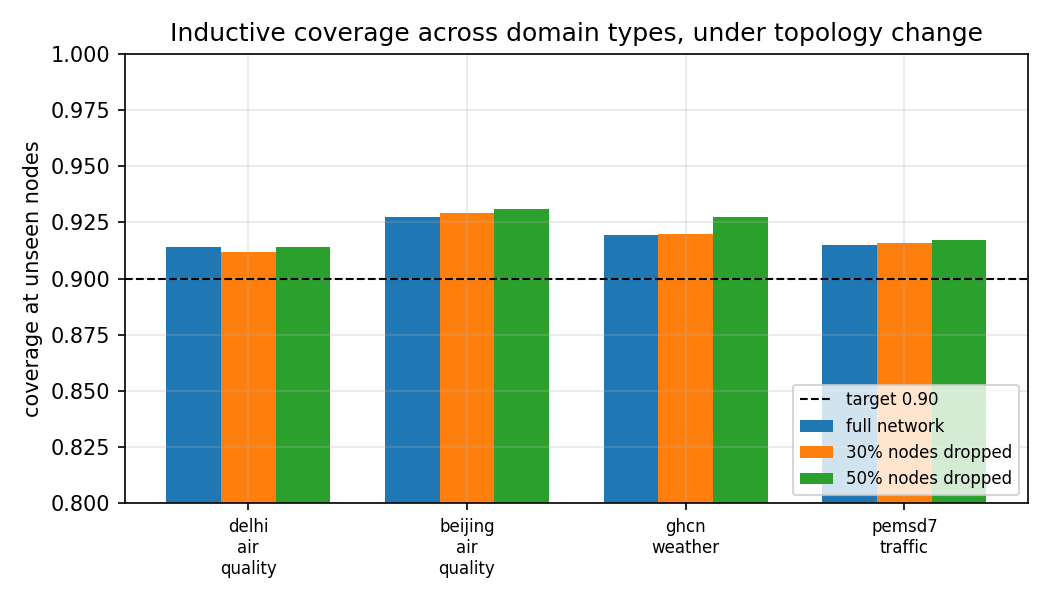
\includegraphics[width=\columnwidth]{fig_multidomain_coverage.png}
\caption{Coverage at unseen sensors on four real datasets, at full network and under 30\% and 50\%
sensor dropout. OmniST holds the 90\% target throughout.}
\label{fig:multidomain}
\end{figure}

Coverage at unseen sensors stays at or above 90\% on all four datasets and holds under 30 to 50\%
dropout (Table~\ref{tab:multidomain}, Fig.~\ref{fig:multidomain}). The nearest-neighbor baseline under-covers on three of them
(Beijing 0.869, weather 0.896, traffic 0.887). Against four model-free interpolators (nearest
neighbor, inverse-distance weighting, mean of $k$ nearest, and a Gaussian-kernel kriging-style
predictor), each wrapped in the same conformal procedure, OmniST is the only method at or above
target on every dataset (Table~\ref{tab:baselines}); all four fall to $0.79$--$0.87$ on Beijing. The
interpolators are often tighter, and sometimes better on point MAE, because they
under-cover. Point MAE is mixed: OmniST wins on Delhi, and interpolation wins on the denser networks.
Ablations in the supplementary material show the coverage comes from the coordinate-based inductive
construction rather than from the attention layer or a particular $k$. The guarantee also tracks other
targets: at 80, 90 and 95\% (5 seeds for air quality, 3 for traffic), empirical coverage is within about
3 points of the target in every cell, for example Delhi $0.824/0.915/0.958$; the loosest cell is traffic
at 80\% ($0.773$).

At 228 traffic sensors inductive coverage is 91.9\%. On the full 325-sensor PeMS-BAY network (3 seeds,
scalable $k$-NN) it is $92.1\pm0.0\%$ and stays at or above 92.0\% under 30/50\% dropout, while the
nearest-neighbor baseline reaches 87.0\%. A scalable neighbor index removes the $O(N^2)$ cost of exact
attention; timing results are in the supplementary material.

\subsection{Coverage Under Seasonal Drift}

\begin{table}[htbp]
\caption{Coverage Over Time Under Seasonal Drift (Delhi, Target 90\%, 3 Seeds)}
\centering
\begin{tabular}{lccc}
\toprule
\textbf{Method} & \textbf{Overall} & \textbf{Late window} & \textbf{Width} \\
\midrule
Static split conformal & 0.758 & 0.498 & 95.4 \\
Rolling window       & 0.840 & 0.799 & 127.4 \\
ACI                  & 0.847 & 0.905 & 139.0 \\
\textbf{Rolling-ACI} & \textbf{0.890} & \textbf{0.962} & 170.1 \\
\bottomrule
\multicolumn{4}{l}{\footnotesize Late window = final third of the test year. Width in $\mu$g/m$^3$.} \\
\end{tabular}
\label{tab:temporal}
\end{table}

The spatial guarantee does not carry over to time for free. Calibrating on the first half of the test
year and evaluating on the second, static conformal covers 0.76 overall and only 0.50 in the final
third of the year. Rolling-ACI restores 0.89 overall and 0.96 in the late window, at the cost of wider
intervals; ACI alone is a narrower middle ground (Table~\ref{tab:temporal}, Fig.~\ref{fig:temporal}).

\begin{figure}[htbp]
\centering
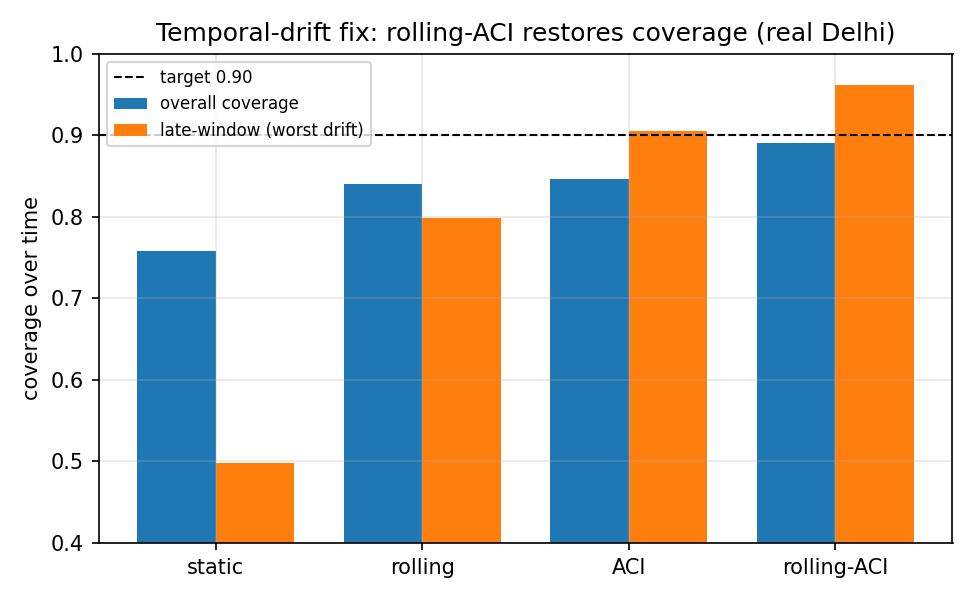
\includegraphics[width=0.9\columnwidth]{fig_temporal_drift.png}
\caption{Coverage over time under seasonal drift on Delhi. Static conformal falls to 0.50 in the late
window; rolling-ACI restores the 90\% target.}
\label{fig:temporal}
\end{figure}

%% ====================================================================
\section{Related Work}
\label{sec:related}

\textbf{Dynamic and inductive forecasting.} Fixed-topology STGCNs~\cite{yu2018stgcn} couple weights to
a sensor count. Expanding-node methods relax this for sensor addition, and inductive kriging
(IGNNK~\cite{ignnk2020}) predicts at unobserved locations; we use it as a baseline. Closest to our
architecture, STFO~\cite{stfo2026} uses coordinate-based aggregation without sensor-specific
parameters to absorb network expansion, and cold-start forecasting at unseen
sensors~\cite{coldstart_unseen2026} conditions a meta-graph on local support. Both target point
prediction under growing networks. OmniST handles removal as well as addition, needs no prompting or
continual-learning machinery, and attaches a coverage guarantee to its inductive forecasts.
Cross-domain spatiotemporal pretraining~\cite{dambast2026} is a different axis that we do not pursue.

\textbf{Conformal prediction on graphs and time series.} Split
conformal~\cite{vovk2005algorithmic,angelopoulos2023conformal} has been extended to correlated time
series~\cite{corel2025}, graph time series~\cite{conformalgraphts2026}, and energy
graphs~\cite{incontextresidual2026}, and~\cite{conformalinductivegnn2024} analyzes the inductive
setting in which new nodes perturb calibration scores. Recent work gives valid conformal prediction
for dynamic GNNs~\cite{validcpdyngnn2024}, non-exchangeable conformal prediction for temporal
GNNs~\cite{nonexchcptgnn2025}, topology-aware intervals for stream networks under
shift~\cite{staci2025}, and online conformalized Gaussian processes on graphs~\cite{conformalgp_online2025}.
These mostly assume a fixed node set whose edges or labels evolve. OmniST targets a different case:
coverage at sensor coordinates with no training history, maintained as sensors are added or removed.
Our online layer follows the spirit of~\cite{conformalgp_online2025,staci2025}; the novelty is its
composition with coordinate-based inductive prediction. Model-free valid spatial
prediction~\cite{validspatial2020} motivates our interpolation baselines.

%% ====================================================================
\section{Limitations}
\label{sec:limitations}

\begin{itemize}
\item \textbf{Marginal, not conditional, coverage.} The guarantee holds on average. Per-sensor
coverage on the irregular traffic network ranges from 0.73 to 0.98; Mondrian (group-conditional)
conformal lifts the worst group from 0.80 to 0.86 but does not reach 0.90 (supplementary material).
Exchangeability of OmniST's inductive scores is argued structurally and checked empirically, not
proved in general.
\item \textbf{Accuracy benchmark.} The comparison with E-STGCN is on Delhi PM$_{2.5}$ only and uses
our reimplementation. Coverage is validated on all four datasets.
\item \textbf{Scale.} Coverage is certified up to 325 real sensors. Thousands of sensors await a larger
real benchmark; synthetic node duplication cannot certify coverage because it breaks exchangeability.
\item \textbf{Coordinates.} For the two traffic datasets, sensor positions are reconstructed from the
released distance adjacency by multidimensional scaling.
\item \textbf{Drift.} Rolling-ACI restores long-run coverage at the price of wider intervals (170
against 95~$\mu$g/m$^3$ on Delhi); its guarantee is asymptotic and marginal, not per step.
\item \textbf{Spatial attention.} Its effect on accuracy at trained sensors is below
0.2~$\mu$g/m$^3$; its value is enabling forecasts and intervals at unseen sensors.
\item \textbf{Seeds.} Cross-domain coverage results use 10 seeds (6 for traffic); the temporal,
inductive-interval and conditional-coverage results use 3.
\end{itemize}

%% ====================================================================
\section{Conclusion}
\label{sec:conclusion}

OmniST is a forecaster for sensor networks that change. Because no component references a global
sensor count, it keeps forecasting when 40\% of stations fail, losing at most 1.1\% accuracy, and it
forecasts at sensors it never trained on. Wrapped in inductive split conformal, it gives intervals at
those unseen sensors whose coverage holds at or above 90\% across four real datasets from three
domains, under 30 to 50\% dropout, and at 325 real sensors, where model-free interpolators fall short
and a fixed-topology baseline cannot produce an output. A rolling adaptive-conformal layer extends the
guarantee over time. The open problems are conditional coverage per sensor and per horizon, and
certifying coverage on real networks with thousands of sensors.

\section*{Data and Code Availability}
All datasets are public: Delhi CPCB PM$_{2.5}$ from the E-STGCN repository~\cite{panja2026estgcn};
Beijing Multi-Site Air Quality from the UCI repository~\cite{zhang2017beijingair}; western-US daily
temperature from NOAA GHCN-Daily; PeMSD7-M traffic from~\cite{yu2018stgcn}; and PeMS-BAY traffic
from~\cite{li2018dcrnn}. The implementation, including the model, loaders for every dataset, each
experiment script, a pinned environment, and an index mapping each reported number to its result
file, is available at \url{\repourl}.

\section*{Acknowledgment}
This research did not receive any specific grant from funding agencies in the public, commercial, or
not-for-profit sectors. The author declares no competing interests; the work was carried out
independently of the author's employment at Sopra Banking Software India, which neither funded nor
directed it. During the preparation of this work the author used Kiro, an AI coding and writing
assistant, to help write and debug experiment code and to draft and edit the manuscript text. The
author reviewed and edited all such content and takes full responsibility for the article.

\bibliographystyle{IEEEtran}
\bibliography{references}

\begin{IEEEbiographynophoto}{Praveg Vashishtha}
is pursuing the Executive M.Tech. degree in the Department of Computer Science and Engineering,
Indian Institute of Technology Patna, India, and is a Senior Software Development Engineer with Sopra
Banking Software India. His research interests include spatiotemporal forecasting for sensor
networks, uncertainty quantification, and regularization for kernel methods.
\end{IEEEbiographynophoto}

\end{document}
